% Templejt .tex fajl nesebicno dao na koriscenje Nikola Milosavljevic
% Ovom prilikom mu se zahvaljujem!

\documentclass[a4paper,12pt]{article}
\usepackage[british]{babel}
\usepackage[]{verbatim}
\usepackage{graphicx}
\usepackage{latexsym}
\usepackage{amssymb}
\usepackage{amsmath}
\usepackage{float}
\usepackage{hyperref}

\newcommand{\razmak}{\vspace{0.2cm}}

% Floor i ceil
\providecommand{\ceil}[1]{\left \lceil #1 \right \rceil }
\providecommand{\floor}[1]{\left \lfloor #1 \right \rfloor }

% Brojanje jednacina
\numberwithin{equation}{subsection}

\title{\Huge \bf Optimizacija i napredne tehnike dinami\v ckog programiranja}

\newtheorem{dfn}{Definicija}[section]
\newtheorem{thm}[dfn]{Teorema}
\newtheorem{lm}[dfn]{Lema}
\newtheorem{pos}[dfn]{Posledica}
\newtheorem{prim}{Primer}

\begin{document}

\renewcommand{\abstractname}{Apstrakt}
\renewcommand{\refname}{Reference}
\renewcommand{\contentsname}{Sadr\v zaj}

\begin{titlepage}
\begin{center}
{\large Prirodno Matemati\v cki Fakultet u Ni\v su}
\end{center}
\vspace{5cm}
\begin{center}
{\Huge \textbf{Optimizacija i napredne tehnike dinami\v ckog programiranja}}
\end{center}
\vspace{7cm}
\large \textbf{Student:} \hspace{8.9 cm} \textbf{Profesor:} \\
\large Ivan Sto\v si\' c \hspace{6.6 cm} Predrag Stanimirovi\' c
\vspace{2.5cm}
\begin{center}{Ni\v s\\
Februar, 2018.}\end{center}
\end{titlepage}

\thispagestyle{headings}

\tableofcontents

\newpage

\pagestyle{headings}

\section{Uvod}

\subsection{Dinami\v cko programiranje}

Dinami\v cko programiranje je tehnika re\v savanja optimizacionih problema i problema prebrojavanja gde se glavni problem re\v sava tako \v sto se identifikuju sli\v cni potproblemi manje veli\v cine, koji se zatim re\v savaju i \v cija se re\v senja kombinuju u re\v senje glavnog problema. Svaki ovako dobijeni potproblem se re\v sava najvi\v se jedanput, nakon \v cega se njegovo re\v senje pamti u memoriji.
\\

Prvi korak u primeni dinami\v ckog programiranja na re\v savanje nekog problema jeste da se identifikuju \textit{potproblemi} tog problema. Najve\' ca instanca me\dj u svim potproblemima jeste \textit{glavni problem}. Najmanje instance su \textit{trivijalni potproblemi}, koji se ne dele dalje na potprobleme i \v cija re\v senja se dobijaju na neki drugi na\v cin. Zatim je neophodno, za svaki potproblem na\' ci relaciju izme\dj u njega i jednog ili vi\v se manjih potproblema. Ova relacija odnosno re\v senje za potproblem je matemati\v cki izraz ili rezultat nekog jednostavnog algoritma u kojem figuri\v su re\v senja manjih potproblema. Ka\v zemo da potproblem $A$ zavisi od potproblema $B$ ako re\v senje potproblema $B$ figuri\v se u izrazu koji je re\v senje potproblema $A$. Da bismo na\v sli re\v senje nekog potproblema neophodno je da prethodno na\dj emo re\v senja za sve potprobleme od kojih on zavisi.
\\

Razmotrimo slede\' ci primer. Neka je glavni problem nala\v zenje broja $k$-elementnih podskupova skupa $\{1, 2, \ldots, n \}$. Identifikujemo slede\' ce potprobleme: Za brojeve $i, j \in \mathbb{N}_0, i \leq n, j \leq k$, na\' ci broj $j$-elementnih podskupova skupa $\{1, 2, \ldots, i \}$. Ozna\v cimo ovaj broj sa $d(i, j)$. Glavni problem je zapravo potproblem gde je $i=n, j=k$. Trivijalni potproblemi su oni gde je $i=0, j>0$, u tom slu\v caju je $d(i, j) = 0$ i problemi gde je $j=0$, gde va\v zi $d(i, j) = 1$. Na\dj imo re\v senje za sve ostale, neka su $i, j > 0$. Posmatrajmo sve $j$-elementne podskupove. Tada svaki od njih ili sadr\v zi element $i$ ili ga ne sadr\v zi. Broj podskupova koji sadr\v ze element $i$ jednak je broju $(j-1)$-elementnih podskupova skupa $\{1, \ldots, i-1 \}$, odnosno $d(i-1, j-1)$. Broj podskupova koji ne sadr\v ze element $i$ jednak je broju $j$-elementnih podskupova skupa od $\{1, \ldots, i-1 \}$, odnosno $d(i-1, j)$. Dakle, dolazimo do slede\' ce formule:
$$
	d(i, j) = d(i-1, j) + d(i-1, j-1)
$$
Ovakve formule \' cemo nazivati \textit{DP vezama}. Argument funkcije $d$ \v cije vrednosti izra\v cunavamo \' cemo nazivati \textit{DP stanjem}. U prethodno razmotrenom primeru DP stanje je element skupa $\{0, \ldots, n\} \times \{0, \ldots, k\}$. DP stanje ne mora nu\v zno biti ure\dj ena $m$-torka brojeva.

\subsection{Slo\v zenost algoritma}

Vreme, odnosno broj koraka i koli\v cina utro\v sene memorije tokom izv\v senja nekog algoritma zavisi od ulaznih parametara. \textit{Veliko O} notacija nam olak\v sava opisivanje i izra\v cunavanje ovih funkecionalnih zavisnosti. Neka je u narednim definicijama domen funkcija $f, g$ skup $\mathbb{N}_0$ a kodomen $\mathbb{R}^{+} \cup \{ 0 \}$.

\begin{dfn}
Skup $O(g)$ defini\v semo kao skup svih funkcija $f$ za koje va\v zi da postoje konstante $c$ i $n_0$ takve da je $f(n) \leq c g(n)$ za svako $n \geq n_0$.
\end{dfn}

Ovu notaciju koristimo kada \v zelimo da opi\v semo gornju granicu neke funkcije, do na proizvod sa konstantom. \v Cesto umesto $f \in O(g)$ pi\v semo i $f = O(g)$. Problem ove notacije je upravo u tome \v sto samo daje gornju granicu pona\v sanja neke funkcije. Zato se uvodi $\Theta$-notacija.

\begin{dfn}
Skup $\Theta(g)$ defini\v semo kao skup svih funkcija $f$ za koje va\v zi da postoje pozitivne konstante $c_1, c_2$ i $n_0$ takve da je $c_1 g(n) \leq f(n) \leq c_2 g(n)$ za svako $n \geq n_0$.
\end{dfn}

Za algoritam \v ciji je ulazni parametar $n$, \v sto mo\v ze biti broj elemenata niza, broj vrsta matrice, broj \v cvorova grafa, itd. ka\v zemo da ima vremensku slo\v zenost $\Theta(g(n))$ ako je $f$, gde je $f(n)$ broj elementarnih koraka tokom izvr\v senja algoritma, u skupu $\Theta(g)$. Sli\v cno defini\v semo memorijsku slo\v zenost preko broja iskori\v s\' cenih elementarnih memorijskih lokacija npr. bajtova ili bitova.

\section{Optimizacija DP algoritama}

Algoritmi dinami\v ckog programiranja mogu da se optimizuju u zavisnosti od problema i DP veze. U ovom odeljku razmotri\' cemo neke od strategija optimizacije.

\subsection{Optimizacija memorije} \label{sec:optmem}

Da bi se izra\v cunalo re\v senje glavnog problema neophodno je izra\v cunati re\v senja nekih potproblema. Me\dj utim, vrlo \v cesto je slu\v caj da nam nisu u svakom trenutku potrebna sva re\v senja do tog trenutka izra\v cunatih potproblema.

Razmotrimo ponovo primer dat u uvodnoj sekciji. Skup stanja je $\{0, \ldots, n\} \times \{0, \ldots, k\}$ a DP veza je
$$
	d(i, j) = d(i-1, j) + d(i-1, j-1)
$$
Primetimo da je broj iskori\v s\' cenih memorijskih lokacija $\Theta(nk)$. Ako posmatramo DP vezu, uo\v cavamo da sve vrednosti $d(n, \cdot)$ mo\v zemo izra\v cunati ako poznajemo sve vrednosti $d(n-1, \cdot)$. Ova \v cinjenica nas navodi na slede\' cu strategiju optimizacije: U svakom trenutku dr\v zimo samo vrednosti $d(i, \cdot)$ i $d(i-1, \cdot)$, odnosno samo dve susedne vrste matrice. Sledi efikasna implementacija ovog pobolj\v sanog algoritma. Nadalje, sve implementacije bi\' ce date u programskom jeziku C++14, ako nije druga\v cije navedeno. Pretpostavlja se da su uklju\v cene odgovaraju\' ce standardne biblioteke.

\begin{figure}[H]
\begin{verbatim}
int brojSkupova(int n, int k) {
    vector<int> d[2];
    d[0].resize(k+1, 0);
    d[1].resize(k+1);
    d[0][0] = 1;
    for (int i=1; i<=n; i++) {
        d[i%2][0] = 1;
        for (int j=1; j<=k; j++)
            d[i%2][j] = d[(i-1)%2][j] + d[(i-1)%2][j-1];
    }
    return d[n%2][k];
}
\end{verbatim}
\end{figure}

U op\v stem slu\v caju, \v zelimo da podelimo sva DP stanja na $m$ slojeva, gde
\' ce za izra\v cunavanje re\v senja u $i$-tom sloju biti dovoljne vrednosti samo iz slojeva $i, i-1, \ldots, i-l$, gde je $l$ mala konstanta. U tom slu\v caju memorijska slo\v zenost se mo\v ze smanjiti na $O(P)$, gde je $P$ maksimalni broj elemenata u jednom sloju. U prethodnom primeru koristimo samo dva sloja, svaki sloj se sastoji od $k+1$ elemenata pa je memorijska slo\v zenost $O(k)$, odnosno ta\v cno $\Theta(k)$.

\subsection{Upotreba pomo\' cnih struktura podataka}

Kod pojedinih problema izraz u DP vezi mo\v ze uklju\v civati veliki broj manjih DP stanja, odnosno, njihov broj mo\v ze biti i nekonstantan. Primer je problem nala\v zenja najve\' ceg rastu\' ceg podniza. Neka je ulaz $a_1, \ldots, a_n$ niz razli\v citih brojeva. Potrebno je na\' ci podskup $I = \{ i_1, i_2, \ldots, i_k \}$ skupa $\{ 1, \ldots, n \}$ takav da se maksimizuje $|I| = k$ i va\v zi $a_{i_1} < a_{i_2} < \ldots < a_{i_k}$ i $i_1 < i_2 < \ldots < i_k$. Ovaj problem ima jednostavno DP re\v senje. Neka je $d_i$ veli\v cina najve\' ceg skupa $I$ koji sadr\v zi element $i$ i neke od elemenata iz skupa $\{ 1, \ldots, i-1 \}$. Re\v senje glavnog problema je onda $\max \{ d_1, \ldots, d_n \}$, po\v sto se svaki podniz mora zavr\v savati na nekoj od ovih $n$ pozicija. Postoji jedan trivijalni potproblem $d_1 = 1$, a za $i>1$ va\v zi:
\begin{equation} \label{eq:lis}
	d_i = 1 + \max_{j<i, a_j < a_i} \{ d_j \}
\end{equation}
Ukoliko takvo $j$ ne postoji, onda je $d_i = 1$. Primetimo da direktna implementacija ove DP veze daje algoritam vremenske slo\v zenosti $\Theta(n^2)$.
\\

Me\dj utim, mo\v zemo iskoristiti augmentovano balansirano binarno stablo da ubrzamo izra\v cunavanje izraza u jedna\v cini (\ref{eq:lis}). Pomenuta struktura podataka se pona\v sa kao sortirani re\v cnik odnosno sortirani niz parova $(k_i, v_i)$, gde je $k$ jedinstveni klju\v c a $v$ uskladi\v stena vrednost. Stablo je augmentnovano dodatnom operacijom \texttt{getRange(l, r)} koja nalazi vrednost agregatne funkcije $f(v_x, \ldots, v_y)$ na proizvoljnom zadatom opsegu klju\v ceva $l \leq k_x, \ldots, k_y < r$. U na\v sem slu\v caju agregatna funkcija je maksimum brojeva. Sve operacije (ubacivanje, brisanje, \texttt{getRange}) rade u slo\v zenosti $O(\log W)$, gde je $W$ trenutni broj elemenata u stablu. U trenutku pre ra\v cunanja vrednosti $d_i$ u stablu \v cuvamo parove $(a_j, d_j)$ za sve $j < i$. Zatim, pozovemo funkciju \texttt{getRange} sa argumentima $l = -\infty, r = a_i$. Ova funkcija nam vra\' ca maksimalnu uskladi\v stenu vrednost (drugi element ure\dj enog para) za sve klju\v ceve koji su manji od $a_i$, odnosno vra\' ca upravo $q = \max_{j<i, a_j < a_i} \{ d_j \}$. Dodatno proveravamo da li je ovaj skup klju\v ceva prazan, u tom slu\v caju postavljamo $q = 0$. Kona\v cno, postavljamo $d_i = q + 1$ u skladu sa (\ref{eq:lis}). Nakon izra\v cunavanja $d_i$ dodajemo par $(a_i, d_i)$ u stablo. Kako operacije dodavanja u stablo i \texttt{getRange} imaju vremensku slo\v zenost $O(\log n)$, ceo algoritam ima slo\v zenost $O(n \log n)$.
\\

\subsection{Optimizacija pomo\' cu linearnih funkcija}

Posmatrajmo jedodimenzione probleme kod kojih DP veza uklju\v cuje sve prethodne potprobleme. Neka je DP veza takva da se mo\v ze svesti na tra\v zenje vrednosti $\max_{j<i} \{ f_j(x_i) \}$ (ili minimuma), gde su $f_j$ linearne funkcije, \v ciji koeficijent pravca i konstanta se mogu dobiti tek nakon izra\v cunavanja vrednosti $d_j$.
\\

Sledi primer ovakvog problema. Neka postoji $n$ trka\v ca, koji u po\v cetku svi stoje u mestu na pozicijama $0 < x_1 < x_2 < \ldots < x_n$. Za svakog trka\v ca poznato je vreme potrebno da pre\dj e jedini\v cno rastojanje $s_i$ i vreme zagrevanja $t_i$ - ovo je vreme koje mu je potrebno od trenutka kada primi \v stafetu do trenutka kada po\v cne da tr\v ci. Nijedan trka\v c ne sme da tr\v ci ukoliko ne nosi \v stafetu i svaki trka\v c mo\v ze tr\v cati samo ulevo. U po\v cetku se \v stafeta nalazi kod $n$-tog trka\v ca. Koliko je najmanje vremena potrebno da se \v stafeta dostavi na poziciju $x = 0$?
\\

Neka je $d_i$ minimalno vreme potrebno da $i$-ti trka\v c dostavi \v stafetu na poziciju $x = 0$ od trenutka kada primi \v stafetu. Dodatno defini\v semo trivijalni potproblem $d_0 = 0$ i postavljamo $x_0 = 0, t_0 = 0$. Neka je $i > 0$. Tada $i$-ti trka\v c treba da izabere kom trka\v cu \' ce dostaviti \v stafetu, ili \' ce je odneti skroz do cilja. Oba slu\v caja opisana su jednom DP vezom:
\begin{equation} \label{eq:lin}
	d_i = t_i + \min_{0 \leq j < i} \{ d_j + s_i(x_i-x_j) \}
\end{equation}
Glavni problem je ra\v cunanje $d_n$. Ponovo, pravolinijska implementacija algoritma koji koristi ovu DP vezu ima vremensku slo\v zenost $\Theta(n^2)$. Zapi\v simo jedna\v cinu (\ref{eq:lin}) na druga\v ciji na\v cin:
$$
	d_i = t_i + \min_{0 \leq j < i} \{ d_j + s_i x_i - s_i x_j \}
$$
Kako $s_i x_i$ ne zavisi od $j$ mo\v ze da iza\dj e ispred minimuma:
$$
	d_i = t_i + s_i x_i + \min_{0 \leq j < i} \{ d_j - s_i x_j \}
$$
Odnosno, ako defini\v semo $f_j(z) = d_j - z x_j$:
$$
	d_i = t_i + s_i x_i + \min_{0 \leq j < i} \{ f_j(s_i) \}
$$
Sada smo problem sveli na odr\v zavanje skupa $Q$ linearnih funkcija, sa operacijom dodavanja linearne funkcije i tra\v zenjem $\min_{f \in Q} f(x)$ za zadato $x$. Odr\v zava\' cemo za svaku funkciju $f_i$ u skupu $Q$, skup brojeva $M_i \subseteq \mathbb{R}$ za koji va\v zi da je $f_i(x)$ najmanja vrednost od svih $f_j(x), f_j \in Q$.
\\

Doka\v zimo da je skup $M_i$ jednak nekom, mo\v zda beskona\v cnom ili praznom intervalu u $\mathbb{R}$. Ozna\v cimo sa $P_{i,j}$ skup svih realnih brojeva $x$ takvih da je $f_i(x) < f_j(x)$. Kako su funkcije $f_i, f_j$ linearne, napi\v simo ih u obliku $f_i(x) = k_i x + b_i, f_j(x) = k_j x + b_j$. Ukoliko je $k_i = k_j$, imamo dva podslu\v caja: Ako je $b_i < b_j$, tada je za svako $x, f_i(x) < f_j(x)$ pa je $P_{i, j} = (-\infty, +\infty)$. U suprotnom je $P_{i,j} = \emptyset$. Neka je sada $k_i \neq k_j$. Tada je $f_i(x) = f_j(x)$ za $x = \frac{b_j-b_i}{k_i-k_j} = x_0$. Ukoliko je $k_i < k_j$, $P_{i, j}$ bi\' ce jednak $(-\infty, x_0)$, u suprotnom $(x_0, +\infty)$, \v cime smo dokazali tvr\dj enje.
\\

Kako je $M_i = \bigcap_{j \neq i} P_{i,j}$, odnosno presek kona\v cno mnogo intervala, i $M_i$ je interval. Primetimo i da su intervali $M_i$ disjunktni. Iz ovog razloga mo\v zemo da \v cuvamo sve neprazne intervale $M_i$ u rastu\' cem redosledu po levom kraju ili po desnom (svejedno je, po\v sto se ne seku). Primetimo da se u ovakvom ure\dj enju $M_i$ mo\v ze na\' ci pre $M_j$ samo ukoliko je $k_i > k_j$.  Tako\dj e, primetimo da je $\mathbb{R} \setminus \bigcup M_i$ kona\v can skup, odnosno, unija $M_i$ pokriva celu realnu pravu osim u kona\v cno mnogo ta\v caka.
\\

\begin{center}
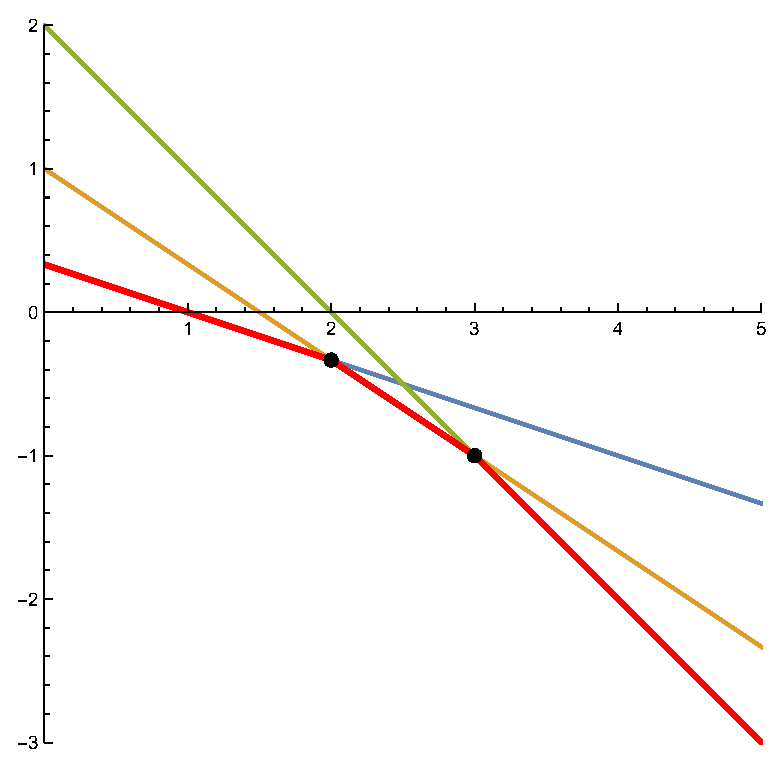
\includegraphics[scale=0.7]{2-3-1.eps}
\\
\textit{Figura 2.3.1: Prikaz intervala minimalnosti $M_i$}
\end{center}

Opi\v simo sada algoritam za nala\v zenje $\min_{f \in Q} \{ f(x) \}$. Jednostavno, binarnom pretragom nalazimo interval $M_i$ u nizu sortiranih intervala i vra\' camo $f_i(x)$. Slo\v zenost je $O(\log |Q|)$.
\\

Opi\v simo zatim algoritam za dodavanje nove funkcije $f_i(x) = k_i x + b_i$. U op\v stem slu\v caju, algoritam je slo\v zeniji i zahteva da se kolekcija $Q$ \v cuva u balansiranom binarnom stablu. Opisa\' cemo jednostavniju verziju gde pretpostavljamo da je $k_i < k_j$ za svako $f_j(x) = k_j x + b_j$ gde je $f_j \in Q$. Drugim re\v cima, dodajemo funkcije u opadaju\' cem redosledu koeficijenata pravaca. Kod velikog broja problema koji se re\v savaju ovom metodom va\v zi upravo ova pretpostavka -- takav je i problem koji je dat na po\v cetku sekcije -- koeficijent pravca $i$-te funkcije koja se dodaje je $-x_i$, a $x_i$ je rastu\' ci niz.
\\

Algoritam je jednostavan: ra\v cuna se presek nove funkcije sa starim intervalima $M_i$ i ovi intervali se po potrebi smanjuju ili izbacuju. U slu\v caju da nova funkcija ima manji koeficijent pravca od svih trenutno uba\v cenih funkcija, svi promenjeni ili izba\v ceni intervali \' ce se nalaziti na kraju ure\dj enog niza, i pritom \' ce najvi\v se jedan biti smanjen, dok \' ce svi ostali (desno od njega) biti izba\v ceni. Dakle, algoritam se sastoji od toga da izbacujemo intervale sa desnog kraja dokle god se oni celi nalaze iznad nove funkcije, a prvi put kada interval se\v ce novu funkciju, zamenimo taj interval presekom i dodamo novu funkciju sa desne strane, ka $+\infty$. Vremenska slo\v zenost je $O(n)$ -- $i$-ta operacija dodavanja sastoji se od $O(z_i)$ koraka, gde je $z_i$ broj izba\v cenih intervala u $i$-tom koraku. Kako svaki interval mo\v ze biti izba\v cen najvi\v se jednom, vremenska slo\v zenost je $O(n)$.

\begin{center}
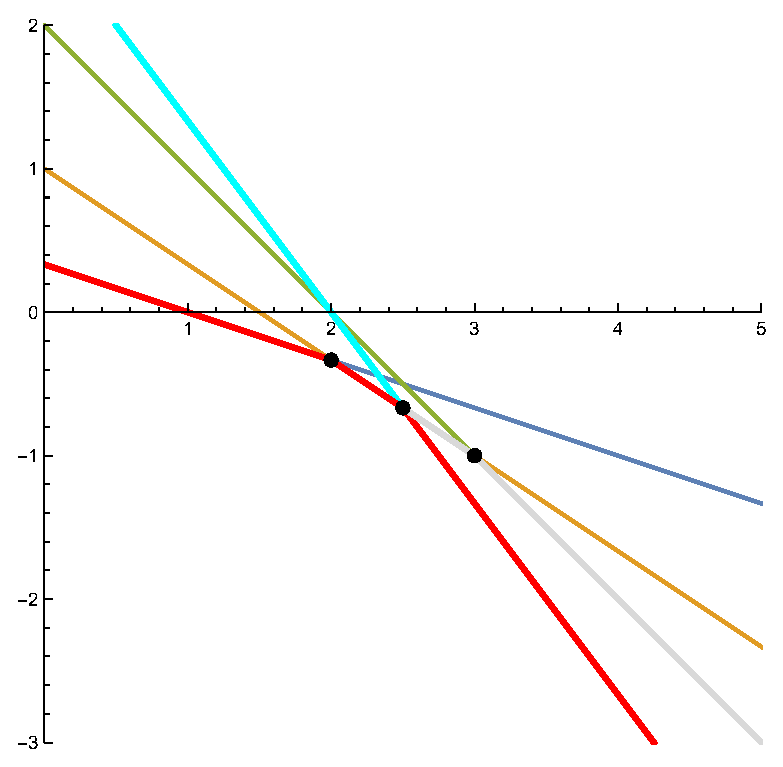
\includegraphics[scale=0.7]{2-3-2.eps}
\\
\textit{Figura 2.3.2: Dodavanje nove funkcije. Nova funkcija obojena je cijan. Izba\v ceni intervali su svetlo-sivi}
\end{center}

Izra\v cunajmo i vremensku slo\v zenost. Imamo $O(n)$ binarnih pretraga, svaka ima vremensku slo\v zenost $O(\log n)$ i pomenuto je da sva dodavanja zajedno imaju ukupnu vremensku slo\v zenost $O(n)$, pa je kona\v cna vremenska slo\v zenost $O(n \log n)$, \v sto je zna\v cajno ubrzanje u odnosu na polaznu slo\v zenost $\Theta(n^2)$.

\subsection{Podeli-pa-vladaj optimizacija}

Posmatrajmo probleme kod kojih je data funkija cene $c(i, j), i \leq j$, za koju va\v zi $c(i,i)=0$ i $c(i, j) > 0$, kada je $i<j$. (koristi\' cemo i zapis $c_{i,j}$) i broj $k$, a potrebno je na\' ci niz indeksa $0 \leq x_1 \leq x_2 \leq \ldots \leq x_k \leq n$ takav da se minimizuje $c(0, x_1) + c(x_1, x_2), \ldots + c(x_{k-1}, x_k) + c(x_k, n)$. Jasno je da se ovaj problem u op\v stem slu\v caju mo\v ze re\v siti slede\' cim algoritmom dinami\v ckog programiranja:
\\

Neka je $d_{i, j}$ minimalni zbir koji se mo\v ze dobiti od svih izraza oblika $c(0, x_1) + c(x_1, x_2) + \ldots + c(x_{i-1}, x_i) + c(x_i, j)$. Re\v si\' cemo $d_{i, j}$ za svako $0 \leq i \leq k$ i $0 \leq j \leq n$. Glavni problem je nala\v zenje vrednosti $d(k, n)$. Trivijalni potproblemi su oni gde je $i = 0$ i tada je $d_{0, j} = c_{0, j}$. Za $i > 0$ va\v zi slede\' ca DP veza:
\begin{equation} \label{eq:dnc}
	d_{i, j} = \min_{0 \leq l \leq j} \{ d_{i-1, l} + c_{l, j} \}
\end{equation}
Postoji $O(nk)$ potproblema i svaki re\v savamo u vremenskoj slo\v zenosti $O(n)$, pa je kona\v cna vremenska slo\v zenost algoritma koji direktno implementira ovu DP vezu $O(n^2k)$. 
\\

Me\dj utim, ukoliko funkcija cene $c(i,j)$ zadovoljava odre\dj ene uslove, mogu\' ce je re\v savati potprobleme u boljoj vremenskoj slo\v zenosti. Jedna takva osobina je monotonost: Funkcija $c$ je monotona ako va\v zi $c(i,j) \leq c(i,k)$ i $c(j,k) \leq c(i,k)$ za svako $i<j<k$. Drugim re\v cima, ukoliko se "opseg" funkcije pro\v siri, vrednost ne mo\v ze da se smanji. Drugi uslov koji je od velikog zna\v caja je tzv. nejednakost \v cetvorougla. Ka\v zemo da funkcija $c$ zadovoljava ovu nejednakost ako va\v zi:
\begin{equation} \label{eq:qineq}
	c(i,k)+c(j,l)\leq c(i,l)+c(j,k)
\end{equation}
za svako $i \leq j \leq k \leq l$. Primer funkcije koja je monotona i zadovoljava nejednakost \v cetvorougla je $c(i,j) = (a_i + a_{i+1} + \ldots + a_{j-1})^2$, gde su $a_i$ dati pozitivni brojevi. Iz nejednakosti \v cetvorougla sledi monotonost: ako je $i<j<k$, imamo:
$$
	c(i, j) + c(j, k) \leq c(j, j) + c(i, k)
$$
po\v sto je $c(j,j) = 0$ i $c(j, k) \geq 0$, direktno dobijamo
$$
	c(i, j) \leq c(i, k)
$$
a iz $c(j,j) = 0$ i $c(i, j) \geq 0$ dobijamo
$$
	c(j, k) \leq c(i, k).
$$
Dakle, u odre\dj enom smislu, nejednakost \v cetvorougla uop\v stava monotonost.
\\

Primetimo da se izra\v cunavanje DP veze (\ref{eq:dnc}) mo\v ze izvesti u $k$ koraka, gde se u $i$-tom koraku ra\v cunaju vrednosti $d_{i,\cdot}$, i svaki korak ima vremensku slo\v zenost $O(n^2)$. Ukoliko funkcija $c$ zadovoljava nejednakost \v cetvorougla, jedan sloj se mo\v ze izra\v cunati u vremenskoj slo\v zenosti $O(n \log n)$, na slede\' ci na\v cin. Defini\v simo $p_{i,j}$ kao vrednost indeksa $l$ za koju se dosti\v ze minimalna vrednost u izrazu (\ref{eq:dnc}). Ukoliko ima vi\v se takvih vrednosti, uzimamo najmanju. Klju\v cna observacija je da za $i>0$ i $x<y$ va\v zi $p_{i,x} \leq p_{i,y}$.
\\

Doka\v zimo ovo tvr\dj enje. Pretpostavimo suprotno: $p_{i,x} > p_{i,y}$. Uvedimo oznake: $\alpha = p_{i,x}$ i $ \beta = p_{i,y}$. Primenimo nejednakost \v cetvorougla na indekse $\beta < \alpha \leq x < y$:
$$
	c(\beta, x) + c(\alpha, y) \leq c(\alpha, x) + c(\beta, y)
$$
Po definiciji $\alpha$ kao najmanjeg indeksa koji minimizuje $d_{i-1, \alpha} + c(\alpha, x)$ va\v zi:
$$
	d_{i-1, \alpha} + c(\alpha, x)
		<
	d_{i-1, \beta} + c(\beta, x)
$$
Ako saberemo ovu nejednakost sa prethodnom, nakon kra\' cenja dobijamo
$$
	d_{i-1, \alpha} + c(\alpha, y) < d_{i-1, \beta} + c(\beta, y)
$$
\v sto je u kontradikciji sa izborom $\beta$.
\\

Algoritam koji je opisan u nastavku se oslanja na ovu osobinu monotonosti indeksa $p_{i,j}$. Algoritam odjednom nalazi sve vrednosti $p_{i,j}$, samim tim i $d_{i,j}$, za neki opseg vrednosti $j \in [l,r] = \{ l, l+1, \ldots, r \}$. Implementacija je rekurzivna, kre\' ce se od opsega $[l,r] = [0, n]$. Svaki rekurzivni poziv sadr\v zi i informaciju o tome u kom opsegu $[u, v]$ se mogu kretati vrednosti $p_{i,j}, j \in [l, r]$. Zatim nalazimo vrednost $w = p_{i,m}$, gde je $m = \floor{\frac{l+r}{2}}$, pretragom po celom opsegu $[u,v]$, i odmah izra\v cunavamo $d_{i,m} = d_{i-1, w} + c(w, m)$. Iz monotonosti $p_{i, j}$ znamo da su sve vrednosti $p_{i,j}$ gde je $j \in [l, m-1]$ iz opsega $[u, w]$ i sli\v cno da su sve vrednosti $p_{i,j}$ gde je $j \in [m+1, r]$ iz opsega $[w, v]$. Sledi generi\v cka implementacija algoritma:

\begin{figure}[H]
\begin{verbatim}
void resiSloj(auto& d, auto c, int i,
          int l, int r, int u, int v) {
    if (l > r)
        return;
    int m = (l+r) / 2, w = u;
    for (int j=u+1; j<=v && j<=m; j++)
        if (d[i-1][j] + c(j, m) < d[i-1][w] + c(w, m))
            w = j;
    d[i][m] = d[i-1][w] + c(w, m);
    resiSloj(d, c, i, l, m-1, u, w);
    resiSloj(d, c, i, m+1, r, w, v);
}

void resiSve(auto& d, auto c, int n, int k) {
    for (int j=0; j<=n; j++)
        d[0][j] = c(0, j);
    for (int i=1; i<=k; i++)
        resiSloj(d, c, i, 0, n, 0, n);
}
\end{verbatim}
\end{figure}

Ovde je $d$ objekat poput dvodimenzionalne matrice u koji mogu da se upisuju vrednosti, $c$ je \textit{callback} funkcija koja izra\v cunava cenu. Izra\v cunajmo slo\v zenost ovog algoritma. Pretpostavljamo da se funkcija $c$ izvr\v sava u vremenskoj slo\v zenosti $O(1)$. Slo\v zenost je jednaka $k$ puta slo\v zenost izvr\v savanja jednog sloja -- na\dj imo ovu slo\v zenost. Kako se u svakom rekurzivnom pozivu funkcije \texttt{resiSloj} segment $[l, r]$ polovi, dubina stabla rekurzije je $O(\log n)$. Posmatrajmo zajedno sve pozive na $i$-tom nivou rekurzije. Ovaj nivo se sastoji od ne vi\v se od $2^i$ poziva -- ozna\v cimo ovaj broj sa $g$. Za vrednosti $u_j, v_j$ unutar jednog sloja va\v ze slede\' ce nejednakosti:
$$
	u_1 \leq v_1 \leq u_2 \leq v_2 \leq \ldots u_g \leq v_g
$$
Kako je vremenska slo\v zenost izvr\v senja koda unutar jednog poziva funkcije (bez rekurzivnih poziva) jednaka $O(v-u)$, u zbiru, vremenska slo\v zenost bi\' ce jednaka $O(\sum(v_i-u_i) + g) = O(n + g) = O(n)$. Kako ima $\log n$ nivoa, ukupna slo\v zenost jednog sloja je $O(n \log n)$, a celog algoritma $O(kn\log n)$.

\subsection{Knutova optimizacija}

Posmatrajmo probleme \v cija je DP veza oblika:
\begin{equation} \label{eq:knuthdp1}
	d_{i, j} = \min_{i < k < j} \{ d_{i, k} + d_{k, j} + c(i, j) \}
\end{equation}
za $0 \leq i, j \leq n$ i $j-i \geq 2$. Trivijalni potproblemi su $d_{i,i+1} = c(i, i+1)$ za $0 \leq i < n$ a cilj nam je da izra\v cunamo vrednost $d_{0, n}$. Direktna implementacija algoritma koji koristi ovu DP vezu ima vremensku slo\v zenost $\Theta(n^3)$, dok je memorijska slo\v zenost $\Theta(n^2)$. Ukoliko za funkciju $c$ va\v zi nejednakost \v cetvorougla (\ref{eq:qineq}), mogu\' ce je ubrzati algoritam. Ozna\v cimo sa $p_{i,j}$ najmanju vrednost $k$ koja minimizuje izraz (\ref{eq:knuthdp1}). Tada va\v zi slede\' ca nejednakost \cite{knuthquad}:
\begin{equation} \label{eq:knuthineq}
	p_{i,j-1} \leq p_{i, j} \leq p_{i+1, j}
\end{equation}
Ovo nam omogu\' cava da za svako $i,j$ vrednost $k$ tra\v zimo na  manjem opsegu. Sledi generi\v cka implementacija pobolj\v sane verzije algoritma.
\\

\begin{figure}[H]
\begin{verbatim}
void resiKnuth(auto& d, auto& p, auto c, int n) {
    for (int i=0; i<n; i++) {
        d[i][i+1] = c(i, i+1);
    }
    for (int i=n-2; i>=0; i--) {
        d[i][i+2] = c(i, i+1) + c(i+1, i+2) + c(i, i+2);
        p[i][i+2] = i+1;
        for (int j=i+3; j<=n; j++) {
            int& w = p[i][j] = p[i][j-1];
            for (int k = p[i][j-1]+1; k <= p[i+1][j]; k++)
                if (d[i][k] + d[k][j] < d[i][w] + d[w][j])
                    w = k;
            d[i][j] = d[i][w] + d[w][j] + c(i, j);
        }
    }
}
\end{verbatim}
\end{figure}

Sli\v cno kao u prethodnoj sekciji, $d, p$ su objekti poput dvodimenzionalne matrice u koje mogu da se upisuju vrednosti, dok je $c$ je \textit{callback} funkcija koja izra\v cunava cenu. Memorijska slo\v zenost ostaje $\Theta(n^2)$. Izra\v cunajmo vremensku slo\v zenost ovog algoritma. Grupi\v simo iteracije spoljne dve for-petlje $(i, j)$ po vrednosti $g = j-i$. Vreme izvr\v senja za $g = 1$ je $O(n)$. Za $g \geq 2$ u vremenu izvr\v senja dominira unutra\v snja for-petlja. Ukupan broj iteracija koje izvr\v si ova for-petlja u okviru grupe $g$ iznosi
\begin{align}
 & \quad \sum_{i=0}^{n-g} (p_{i+1, i+g} - p_{i, i+g-1}) \nonumber \\
=& \quad \sum_{i=0}^{n-g} p_{i+1, i+g} - \sum_{i=0}^{n-g} p_{i, i+g-1} \nonumber \\
=& \quad \sum_{i=1}^{n-g+1} p_{i, i+g-1} - \sum_{i=0}^{n-g} p_{i, i+g-1} \nonumber \\
=& \quad p_{n-g+1, n} - p_{0, g-1} \nonumber \\
\leq & \quad n - 0 \nonumber \\
\end{align}
\v sto je $O(n)$. Dakle, ukupna vremenska slo\v zenost izvr\v senja je $O(n^2)$, odnosno, po\v sto svakako imamo dve for-petlje po $i,j$, ta\v cno $\Theta(n^2)$.
\\

Primer problema \v cija DP veza ima oblik \textit{nalik na} (\ref{eq:knuthdp1}) jeste problem nala\v zenja optimalnog binarnog stabla pretrage: Postoji $n$ jedinstvenih klju\v ceva, ure\dj enih u rastu\' cem redosledu -- $i$-tom klju\v cu ($1 \leq i \leq n$) pridru\v zena je verovatno\' ca $p_i$ da \' ce u stablu biti tra\v zen ba\v s taj klju\v c. Va\v zi $\sum_{i=1}^{n} p_i = 1$. Potrebno je prona\' ci binarno stablo pretrage koje minimizuje o\v cekivano vreme tra\v zenja klju\v ca, odnosno, ako je \v cvor $i$ na dubini $b_i \geq 1$, treba minimizovati izraz $\sum_{i=1}^{n} b_ip_i$. Defini\v simo $d_{i,j}$ kao minimalno o\v cekivano vreme tra\v zenja klju\v ceva ako formiramo samo stablo od klju\v ceva \v ciji su redni brojevi $i,i+1,\ldots,j$. Za $i=j$ va\v zi $d_{i,j} = p_i$ -- koren se nalazi na dubini $1$. Za $d_{i,j}$ gde je $i>j$ defini\v semo vrednost $0$ -- ovaj slu\v caj odgovara stablu bez \v cvorova. U op\v stem slu\v caju, od \v cvorova $i,i+1,\ldots,j$ treba odabrati koren $k$ i rasporediti ostale \v cvorove u levo i desno podstablo. \v Cvorove sa indeksima manjim od $k$ moramo staviti u levo, a ostale u desno podstablo da bismo dobili binarno stablo pretrage. Dakle, treba minimizovati vrednost izraza
\begin{equation} \label{eq:knppd}
	\sum_{u=i}^{k-1} b_u p_u + p_k + \sum_{u=k+1}^{j} b_u p_u
\end{equation}
Kako je dubina \v cvorova u levom podstablu za $1$ ve\' ca od dubine koju bi ti \v cvorovi imali u slu\v caju da je to celo stablo, suma sa leve strane $\sum_{u=i}^{k-1} b_u p_u$ je za ta\v cno $\sum_{u=i}^{k-1} p_u$ ve\' ca od sume koja bi se dobila u slu\v caju da je to celo stablo, pa isti raspored \v cvorova istovremeno minimizuje oba izraza. Iz ovoga sledi da je zapravo minimalna vrednost sume $\sum_{u=i}^{k-1} b_u p_u$ jednaka $d_{i, k-1} + \sum_{u=i}^{k-1} p_u$, pa je minimalna vrednost izraza (\ref{eq:knppd}) jednaka
$$
	d_{i,j} = \min_{i \leq k \leq j} \{ d_{i, k-1} + d_{k+1, j} + 
		\sum_{u=i}^{k-1} p_u + \sum_{u=k+1}^{j} p_u + p_k \}
$$
odnosno
\begin{equation} \label{eq:knpd}
	d_{i,j} = \min_{i \leq k \leq j} \{ d_{i, k-1} + d_{k+1, j} + 
		\sum_{u=i}^{j} p_u\}
\end{equation}
\\

Primetimo da ova DP veza nema oblik identi\v can obliku (\ref{eq:knuthdp1}). Sre\' com, za ovaj problem va\v zi nejednakost (\ref{eq:knuthineq}) \cite{knuthtree}, pa je gore opisani algoritam i dalje primenljiv, uz manje modifikacije. Funkciju $c(i, j) = \sum_{u=i}^{j} p_u$ mo\v zemo ra\v cunati u vremenskoj slo\v zenosti $O(1)$ pomo\' cu pomo\' cnog niza \textit{prefiksnih suma}.

\subsection{Binarno stepenovanje}

Posmatrajmo probleme kod kojih DP veza ima slede\' ci oblik:
\begin{equation} \label{eq:binstep}
	d_{i, j} = \sum_{k=1}^{n} A_{j, k} \cdot d_{i-1, k}
\end{equation}
za $1 \leq j \leq n$, $1 \leq i \leq m$, a trivijalni potproblemi su oni gde je $i=0, 1 \leq j \leq n$, gde je $d_{0, j} = b_j$. Cilj nam je da izra\v cunamo vrednosti $d_{m, \cdot}$. Postoji $nm$ netrivijalnih vrednosti i svaku ra\v cunamo u slo\v zenosti $O(n)$, pa je ukupna vremenska slo\v zenost direktne implementacije $O(n^2 m)$. Memorijska slo\v zenost (ne ra\v cunaju\' ci matricu $a$) se mo\v ze smanjiti na $O(n)$ pomo\' cu tehnike optimizacije memorije opisane u sekciji \ref{sec:optmem}. Jasno je da DP veza (\ref{eq:binstep}) odgovara proizvodu matrice $A$ i vektora $d_{i-1}$:
$$
	d_i = A \cdot d_{i-1}
$$
Kako je $d_0 = b$ i mno\v zenje matrica je asocijativno, va\v zi
$$
	d_i = A^i \cdot b
$$

Mogu\' ce je primeniti tehniku binarnog stepenovanja da bi se direktno izra\v cunala matrica $A_m$, a samim tim i vektor $d_m = A_m \cdot b$. Naime, $m$-ti stepen ($m \in \mathbb{N}$) nekog broja, matrice, ili elementa proizvoljne polugrupe $a^m$ se mo\v ze izra\v cunati pomo\' cu slede\' ceg rekurzivnog algoritma:

\begin{itemize}
\item Ukoliko je $x=1$, vrati $a$.
\item Ukoliko je $x$ paran broj, izra\v cunaj $q = a^\frac{x}{2}$ i vrati $q^2$
\item Ukoliko je $x>1$ neparan broj, izra\v cunaj $q = a^{x-1}$ i vrati $aq$.
\end{itemize}

Kako posle svaka dva rekurzivna koraka vrednost postane bar duplo manja, broj mno\v zenja je $O(2 \log_2m) = O(\log m)$. Mno\v zenje dve matrice se mo\v ze realizovati u vremenskoj slo\v zenosti $O(n^3)$ naivnim algoritmom, a postoji i algoritam slo\v zenosti $O(n^{2.3729})$ \cite{matrixmul}, tako da je kona\v cna vremenska slo\v zenost $O(n^{2.3729} \log m)$, \v sto je pogodnije za veoma velike vrednosti $m$.
\\

Primer problema koji se mo\v ze re\v siti na ovaj na\v cin je problem brojanja \v setnji du\v zine $m$ u grafu zadatog matricom susedstva $A$, od \v cvora $u$ do \v cvora $v$. Za po\v cetni vektor $b$ uzimamo $b_u = 1$ i $b_i = 0, i \neq u$. Kona\v cno re\v senje je polje $d_{m, v}$ vektora $d_m = A^m \cdot b$.

\section{Napredne DP tehnike}

U ovoj glavi bavi\' cemo se problemima \v cija formulacija preko dinami\v ckog programiranja nije o\v cigledna, kao i problemima kod kojih manje o\v cigledna formulacija daje daleko efikasniji algoritam.

\subsection{DP sa nekompletnim stanjima}

Posmatrajmo slede\' ci problem:
\\

Postoji $n$ studenata, $i$-ti ($1\leq i \leq n$) ima efikasnost $a_i$, i dat je broj $k$. Potrebno je na\' ci broj particija skupa studenata tj. broj familija $P$ tako da va\v zi:
\begin{itemize}
\item $\bigcup_{X \in P} X = \{1,\ldots,n\}$
\item $\forall X, Y \in P, X \neq Y \implies X \cap Y = \emptyset$
\item $\sum_{X \in P} \delta(X) \leq k$
\end{itemize}
gde je $\delta(X)$ disbalans skupa studenata, $\delta(X) = \max_{i \in X} \{ a_i \} - \min_{i \in X} \{ a_i \}$. Vrednosti $a_i$ su prirodni brojevi i va\v zi $a_i \leq A$.
\\

Za po\v cetak, sortirajmo niz $a$. Neka je $d(i, j, l)$ broj takvih particija koriste\' ci prvih $i$ studenata, takvih da ima ukupno $j$ \textit{nedovr\v senih} skupova i da je ukupna \textit{projektovana} suma disbalansa jednaka $l$. Ukoliko nema nedovr\v senih skupova, ova projektovana suma disbalansa jednaka je ukupnoj sumi disbalansa (za sve dovr\v sene tj. kompletne skupove). Svaki nedovr\v sen skup je neprazan i doprinosi projektovanoj sumi disbalansa sa $-a_x$, gde je $x$ indeks prvog studenta koji je dodat u taj skup. Po\v sto su studenti sortirani, ovo \' ce upravo biti minimalno $a_x$ tog skupa. U $i$-tom potezu mo\v zemo izabrati jednu od \v cetiri opcije:
\begin{enumerate}
\item Zapo\v cinjemo nov nekompletan skup. Ukupna projektovana suma (vrednost $l$) se pove\' cava za $-a_i$, a $j$ (broj nekompletnih skupova) se pove\' cava za jedan.
\item Zatvaramo neki ranije otvoren skup. Kako je $a_i$ najve\' ca vrednost tog skupa, $l$ se pove\' cava za $a_i$ a broj otvorenih skupova se smanjuje za jedan. Ovo mo\v zemo u\v ciniti samo ukoliko je $j > 0$.
\item Dodajemo $a_i$ u novi, zaseban skup koji odmah progla\v savamo zatvorenim. Vrednosti $j,l$ se ne menjaju.
\item Dodajemo $a_i$ u neki od trenutno otvorenih skupova, bez zatvaranja. Ovo mo\v zemo uraditi na $j$ razli\v citih na\v cina. Vrednosti $j,l$ se ne menjaju.
\end{enumerate}

Obrazlo\v zimo stavku 2. Recimo da $i$-tog studenta dodajemo u neki ranije otvoren skup \v cija je minimalna vrednost $a_x$. U trenutku kada smo otvorili taj skup, smanjili smo $l$ za $a_x$. U trenutku zatvaranja pove\' cali smo $l$ za $a_i$, pa smo efektivno pove\' cali $l$ za $a_i - a_x$, \v sto je upravo disbalans ovog skupa.

Nas na kraju zanima vrednost $\sum_{l=0}^{k} d(n, 0, l)$ (na kraju ne sme biti nedovr\v senih skupova). Kako $j$ mo\v ze uzimati vrednosti $0 \leq j \leq n$ a $l$ mo\v ze uzimati vrednosti $-nA \leq l \leq nA$, ima ukupno $O(n^3 A)$ stanja. Svako re\v savamo u $O(1)$ pa je ukupna vremenska slo\v zenost $O(n^3 A)$ \v sto \v cini ovaj algoritam pseudopolinomijalnim, sli\v cno kao poznati algoritmi za problem ranca.

\subsection{DP na povezanim komponentama}

Ova tehnika i njene modifikacije se mogu koristiti kod zadataka koji zahtevaju brojanje permutacija koje zadovoljavaju neku osobinu. Primer je slede\' ci zadatak:
\\

Dat je skup razli\v citih celih brojeva $\{a_1, \ldots, a_n \}$ i prirodan broj $k$. Koliko ima permutacija $\sigma : \{1, \ldots, n\} \rightarrow \{1, \ldots, n\} $ tako da va\v zi:
$$
	\sum_{i=1}^n |a_{\sigma_i} - a_{\sigma_{i+1}}| = k
$$
U ovoj sumi uzimamo da je $\sigma_{n+1} = \sigma_1$. Za brojeve $a_i$ va\v zi $0 \leq a_i \leq A$.
\\

Sli\v cno kao u primeru iz prethodne sekcije, \v zelimo da na\dj emo re\v senje pseudopolinomijalne vremenske slo\v zenosti, odnosno polinomijalne po $n, A$. Definisa\' cemo DP stanje na slede\' ci na\v cin: neka je $d_{i,j,l}$ broj skupova koji opisuju povezane komponente delimi\v cno popunjenih permutacija gde je uba\v ceno $i$ brojeva, ima $j$ povezanih komponenti i ukupna projektovana suma je $l$. Redosled povezanih komponenti u permutaciji nije bitan ali redosled elemenata u povezanoj komponenti jeste. Delimi\v cno popunjena permutacija je svaki niz od $n$ elemenata od kojih su $i$ poznati, a ostali su nepoznati. Povezana komponenta je niz uzastopnih poznatih vrednosti -- na primer, $(1, ?, 2, ?, 3)$ ima dve povezane komponente jer uzimamo da su $3,1$ susedni. Ovo je posledica oblika sume. Dalje, za projektovanu sumu uzimamo sumu apsolutnih razlika za sve susedne parove poznatih brojeva i dodajemo $-1$ puta suma svih poznatih brojeva koji se nalaze na rubu povezane komponente. Ukoliko se poznat broj nalazi u komponenti koja sadr\v zi samo njega (nema suseda), onda taj broj ra\v cunamo dvaput. Klju\v cna ideja jeste da brojeve ubacujemo u permutaciju u rastu\' cem poretku. Posmatrajmo mogu\' ce situacije koje mogu da nastanu dodavanjem novog, $(i+1)$-og broja.
\begin{enumerate}
\item Broj je dodat u novu povezanu komponentu i nema suseda. Ovo je mogu\' ce uraditi na jedan na\v cin ukoliko je $n-i > 2j$, ina\v ce nije mogu\' ce. Ima $n-i$ nepopunjenih mesta od kojih su ta\v cno $2j$ susedi neke postoje\' ce komponente. Vrednost $j$ se pove\' cava za $1$ dok se suma $l$ pove\' cava za $-2a_{i+1}$.
\item Broj je dodat na rub jedne komponente, ali njegovim dodavanjem nisu spojene dve razli\v cite komponente. Ovo je mogu\' ce uraditi na $2j$ na\v cina ukoliko je $n-i > j$. Broj povezanih komponenti se ne menja. Neka je $a_r$ vrednost broja koji je bio na rubu gde je dodat broj $a_{i+1}$. Od sume prvo oduzimamo $-a_r$ odnosno dodajemo $a_r$. Zatim dodajemo $|a_{i+1} - a_r| = a_{i+1} - a_r$, jer brojeve ubacujemo u rastu\' cem redosledu i kona\v cno dodajemo $-a_{i+1}$ jer je sada ovaj broj na rubu. Ukupno, suma \' ce se promeniti za $a_r + a_{i+1} - a_r - a_{i+1} = 0$.
\item Broj spaja dve povezane komponente. Ovo je mogu\' ce uraditi na $j(j-1)$ na\v cina -- to je proizvod broja na\v cina da izaberemo prvu (sa leve strane) i drugu (sa desne strane), redosled je va\v zan. Mora va\v ziti $j>1$. Broj povezanih komponenti se smanjuje za $1$. Ako su $a_p$ i $a_q$ rubni elementi te dve komponente, prvo od sume oduzimamo $-a_p$ i $-a_q$ odnosno dodajemo $a_p+a_q$. Zatim dodajemo $|a_{i+1}-a_p| + |a_{i+1}-a_q|$ odnosno $2a_{i+1}-a_p-a_q$. Ne javljaju se novi rubni elementi. Ukupno, suma $l$ se pove\' cava za $2a_{i+1}$.
\end{enumerate}

Ciljno stanje je ono gde je $i=n, j=1, l=k$. Ra\v cunamo $d_{i,j,l}$ u rastu\' cem redosledu po $i$, rukovode\' ci se gore opisanim postupkom. Trivijalan potproblem, odnosno polazna vrednost je $i=0,j=0,l=0$, gde je $d_{i,j,l} = 1$, postoji samo jedan prazan raspored.
\\

Kako $i$ uzima vrednosti iz skupa $\{ 0, \ldots, n \}$, $j$ iz skupa $\{0, \ldots, \floor{\frac{n}{2}} \}$, a $l$ iz skupa $\{ -2nA, \ldots, 2nA \}$, ima ukupno $O(n^3 A)$ stanja, svako stanje ra\v cunamo u $O(1)$ pa je kona\v cna vremenska slo\v zenost ovog algoritma $O(n^3 A)$.

\section{Zadaci za samostalan rad}

\begin{enumerate}
\item \textbf{\href{http://codeforces.com/problemset/problem/838/E}{[Codeforces 838E]}} Dat je strogo konveksan mnogougao sa $n$ ta\v caka. Na\' ci du\v zinu najdu\v ze izlomljene linije bez samopresecanja \v cija su temena ujedno i temena datog mnogougla. Tra\v zi se re\v senje vremenske slo\v zenosti $O(n^2)$.

\item \textbf{\href{http://codeforces.com/problemset/problem/809/D}{[Codeforces 809D]}} Dat je niz segmenata $[l_i, r_i], 1 \leq i \leq n$, $l_i, r_i \in \mathbb{Z}$. Na\' ci najve\' ci broj $k$ tako da postoje indeksi $1 \leq x_1 < x_2 \ldots < x_k \leq n$ i celi brojevi $y_1 < y_2 < \ldots < y_k$ takvi da je $l_{x_i} \leq y_i \leq r_{x_i}$ za svako $i \in \{1, \ldots, k \}$. Tra\v zi se re\v senje vremenske slo\v zenosti $O(n \log n)$.

\item \textbf{\href{http://codeforces.com/problemset/problem/868/F}{[Codeforces 868F]}} Dat je niz celih brojeva $a_1, \ldots, a_n$ i prirodan broj $k \leq n$. Cena jednog podsegmenta je broj neure\dj enih parova razli\v citih indeksa unutar tog podsegmenta takvih da se na tim pozicijama nalaze jednaki brojevi. Podeliti niz na ta\v cno $k$ podsegmenata tako da je minimizovan zbir cena svih podsegmenata. Tra\v zi se re\v senje vremenske slo\v zenosti $O(n(k + \log n))$.

\item \textbf{\href{http://ceoi.inf.elte.hu/probarch/09/harbingers.pdf}{[CEOI 2009, Harbingers]}} Dato je stablo sa \v cvorovima $\{1, \ldots, n\}$ i korenom u \v cvoru $1$. Data je i du\v zina svake grane (pozitivan broj). U svakom \v cvoru, osim u korenu, nalazi se kurir. Za svakog kurira poznata je njegova brzina i vreme koje mu je potrebno da krene od kad primi poruku. Kuriri mogu da se kre\' cu samo ka korenu stabla. Za svaki od gradova $\{2, \ldots, n\}$ na\' ci najmanje vreme potrebno da poruka stigne do korena. Tra\v zi se re\v senje vremenske slo\v zenosti $O(n \log n)$.

\item \textbf{\href{http://bubblecup.petlja.org/Content/Media/Booklet2016.pdf}{[Bubble Cup 2016 Finals, H]}} Dva igra\v ca igraju igru Nim sa $n$ gomila. Veli\v cine ovih gomila su nezavisne slu\v cajne promenljive, \v cija je raspodela verovatno\' ca data nizom $p_1, \ldots, p_m$ (sve imaju istu raspodelu), verovatno\' ca da neka gomila ima veli\v cinu $i$ je $p_i$. Na\' ci verovatno\' cu da prvi igra\v c ima pobedni\v cku strategiju. Tra\v zi se re\v senje vremenske slo\v zenosti $O(x^2 \log n)$.

\end{enumerate}

\section{Zaklju\v cak}

Savladali smo dinami\v cko programiranje.

\addcontentsline{toc}{section}{Literatura}

\begin{thebibliography}{10}

% 10.1145/1644015.1644032
\bibitem{knuthquad} Bein W, Golin M.J, Larmore L.L, Zhang Y. \textit{The Knuth-Yao quadrangle-inequality speedup is a consequence of total monotonicity}. TALG, vol. 6 (2009)

% 10.1007/BF00264289
\bibitem{knuthtree} Knuth D.E. \textit{Optimum binary search trees}, Acta Informatica, vol. 1 (1971)

% 10.1007/978-3-319-72547-5
\bibitem{finn} Laaksonen A. \textit{Guide to Competitive Programming}, Springer International Publishing (2017)

% 10.1145/2746539.2746554
\bibitem{matrixmul} Ambainis A, Filmus Y, Le Gall F. \textit{Fast Matrix Multiplication: Limitations of the Coppersmith-Winograd Method}. STOC (2015)

\end{thebibliography}

\end{document} 